\documentclass[11pt]{article}

    \usepackage[breakable]{tcolorbox}
    \usepackage{parskip} % Stop auto-indenting (to mimic markdown behaviour)
    

    % Basic figure setup, for now with no caption control since it's done
    % automatically by Pandoc (which extracts ![](path) syntax from Markdown).
    \usepackage{graphicx}
    % Keep aspect ratio if custom image width or height is specified
    \setkeys{Gin}{keepaspectratio}
    % Maintain compatibility with old templates. Remove in nbconvert 6.0
    \let\Oldincludegraphics\includegraphics
    % Ensure that by default, figures have no caption (until we provide a
    % proper Figure object with a Caption API and a way to capture that
    % in the conversion process - todo).
    \usepackage{caption}
    \DeclareCaptionFormat{nocaption}{}
    \captionsetup{format=nocaption,aboveskip=0pt,belowskip=0pt}

    \usepackage{float}
    \floatplacement{figure}{H} % forces figures to be placed at the correct location
    \usepackage{xcolor} % Allow colors to be defined
    \usepackage{enumerate} % Needed for markdown enumerations to work
    \usepackage{geometry} % Used to adjust the document margins
    \usepackage{amsmath} % Equations
    \usepackage{amssymb} % Equations
    \usepackage{textcomp} % defines textquotesingle
    % Hack from http://tex.stackexchange.com/a/47451/13684:
    \AtBeginDocument{%
        \def\PYZsq{\textquotesingle}% Upright quotes in Pygmentized code
    }
    \usepackage{upquote} % Upright quotes for verbatim code
    \usepackage{eurosym} % defines \euro

    \usepackage{iftex}
    \ifPDFTeX
        \usepackage[T1]{fontenc}
        \IfFileExists{alphabeta.sty}{
              \usepackage{alphabeta}
          }{
              \usepackage[mathletters]{ucs}
              \usepackage[utf8x]{inputenc}
          }
    \else
        \usepackage{fontspec}
        \usepackage{unicode-math}
    \fi

    \usepackage{fancyvrb} % verbatim replacement that allows latex
    \usepackage{grffile} % extends the file name processing of package graphics
                         % to support a larger range
    \makeatletter % fix for old versions of grffile with XeLaTeX
    \@ifpackagelater{grffile}{2019/11/01}
    {
      % Do nothing on new versions
    }
    {
      \def\Gread@@xetex#1{%
        \IfFileExists{"\Gin@base".bb}%
        {\Gread@eps{\Gin@base.bb}}%
        {\Gread@@xetex@aux#1}%
      }
    }
    \makeatother
    \usepackage[Export]{adjustbox} % Used to constrain images to a maximum size
    \adjustboxset{max size={0.9\linewidth}{0.9\paperheight}}

    % The hyperref package gives us a pdf with properly built
    % internal navigation ('pdf bookmarks' for the table of contents,
    % internal cross-reference links, web links for URLs, etc.)
    \usepackage{hyperref}
    % The default LaTeX title has an obnoxious amount of whitespace. By default,
    % titling removes some of it. It also provides customization options.
    \usepackage{titling}
    \usepackage{longtable} % longtable support required by pandoc >1.10
    \usepackage{booktabs}  % table support for pandoc > 1.12.2
    \usepackage{array}     % table support for pandoc >= 2.11.3
    \usepackage{calc}      % table minipage width calculation for pandoc >= 2.11.1
    \usepackage[inline]{enumitem} % IRkernel/repr support (it uses the enumerate* environment)
    \usepackage[normalem]{ulem} % ulem is needed to support strikethroughs (\sout)
                                % normalem makes italics be italics, not underlines
    \usepackage{soul}      % strikethrough (\st) support for pandoc >= 3.0.0
    \usepackage{mathrsfs}
    

    
    % Colors for the hyperref package
    \definecolor{urlcolor}{rgb}{0,.145,.698}
    \definecolor{linkcolor}{rgb}{.71,0.21,0.01}
    \definecolor{citecolor}{rgb}{.12,.54,.11}

    % ANSI colors
    \definecolor{ansi-black}{HTML}{3E424D}
    \definecolor{ansi-black-intense}{HTML}{282C36}
    \definecolor{ansi-red}{HTML}{E75C58}
    \definecolor{ansi-red-intense}{HTML}{B22B31}
    \definecolor{ansi-green}{HTML}{00A250}
    \definecolor{ansi-green-intense}{HTML}{007427}
    \definecolor{ansi-yellow}{HTML}{DDB62B}
    \definecolor{ansi-yellow-intense}{HTML}{B27D12}
    \definecolor{ansi-blue}{HTML}{208FFB}
    \definecolor{ansi-blue-intense}{HTML}{0065CA}
    \definecolor{ansi-magenta}{HTML}{D160C4}
    \definecolor{ansi-magenta-intense}{HTML}{A03196}
    \definecolor{ansi-cyan}{HTML}{60C6C8}
    \definecolor{ansi-cyan-intense}{HTML}{258F8F}
    \definecolor{ansi-white}{HTML}{C5C1B4}
    \definecolor{ansi-white-intense}{HTML}{A1A6B2}
    \definecolor{ansi-default-inverse-fg}{HTML}{FFFFFF}
    \definecolor{ansi-default-inverse-bg}{HTML}{000000}

    % common color for the border for error outputs.
    \definecolor{outerrorbackground}{HTML}{FFDFDF}

    % commands and environments needed by pandoc snippets
    % extracted from the output of `pandoc -s`
    \providecommand{\tightlist}{%
      \setlength{\itemsep}{0pt}\setlength{\parskip}{0pt}}
    \DefineVerbatimEnvironment{Highlighting}{Verbatim}{commandchars=\\\{\}}
    % Add ',fontsize=\small' for more characters per line
    \newenvironment{Shaded}{}{}
    \newcommand{\KeywordTok}[1]{\textcolor[rgb]{0.00,0.44,0.13}{\textbf{{#1}}}}
    \newcommand{\DataTypeTok}[1]{\textcolor[rgb]{0.56,0.13,0.00}{{#1}}}
    \newcommand{\DecValTok}[1]{\textcolor[rgb]{0.25,0.63,0.44}{{#1}}}
    \newcommand{\BaseNTok}[1]{\textcolor[rgb]{0.25,0.63,0.44}{{#1}}}
    \newcommand{\FloatTok}[1]{\textcolor[rgb]{0.25,0.63,0.44}{{#1}}}
    \newcommand{\CharTok}[1]{\textcolor[rgb]{0.25,0.44,0.63}{{#1}}}
    \newcommand{\StringTok}[1]{\textcolor[rgb]{0.25,0.44,0.63}{{#1}}}
    \newcommand{\CommentTok}[1]{\textcolor[rgb]{0.38,0.63,0.69}{\textit{{#1}}}}
    \newcommand{\OtherTok}[1]{\textcolor[rgb]{0.00,0.44,0.13}{{#1}}}
    \newcommand{\AlertTok}[1]{\textcolor[rgb]{1.00,0.00,0.00}{\textbf{{#1}}}}
    \newcommand{\FunctionTok}[1]{\textcolor[rgb]{0.02,0.16,0.49}{{#1}}}
    \newcommand{\RegionMarkerTok}[1]{{#1}}
    \newcommand{\ErrorTok}[1]{\textcolor[rgb]{1.00,0.00,0.00}{\textbf{{#1}}}}
    \newcommand{\NormalTok}[1]{{#1}}

    % Additional commands for more recent versions of Pandoc
    \newcommand{\ConstantTok}[1]{\textcolor[rgb]{0.53,0.00,0.00}{{#1}}}
    \newcommand{\SpecialCharTok}[1]{\textcolor[rgb]{0.25,0.44,0.63}{{#1}}}
    \newcommand{\VerbatimStringTok}[1]{\textcolor[rgb]{0.25,0.44,0.63}{{#1}}}
    \newcommand{\SpecialStringTok}[1]{\textcolor[rgb]{0.73,0.40,0.53}{{#1}}}
    \newcommand{\ImportTok}[1]{{#1}}
    \newcommand{\DocumentationTok}[1]{\textcolor[rgb]{0.73,0.13,0.13}{\textit{{#1}}}}
    \newcommand{\AnnotationTok}[1]{\textcolor[rgb]{0.38,0.63,0.69}{\textbf{\textit{{#1}}}}}
    \newcommand{\CommentVarTok}[1]{\textcolor[rgb]{0.38,0.63,0.69}{\textbf{\textit{{#1}}}}}
    \newcommand{\VariableTok}[1]{\textcolor[rgb]{0.10,0.09,0.49}{{#1}}}
    \newcommand{\ControlFlowTok}[1]{\textcolor[rgb]{0.00,0.44,0.13}{\textbf{{#1}}}}
    \newcommand{\OperatorTok}[1]{\textcolor[rgb]{0.40,0.40,0.40}{{#1}}}
    \newcommand{\BuiltInTok}[1]{{#1}}
    \newcommand{\ExtensionTok}[1]{{#1}}
    \newcommand{\PreprocessorTok}[1]{\textcolor[rgb]{0.74,0.48,0.00}{{#1}}}
    \newcommand{\AttributeTok}[1]{\textcolor[rgb]{0.49,0.56,0.16}{{#1}}}
    \newcommand{\InformationTok}[1]{\textcolor[rgb]{0.38,0.63,0.69}{\textbf{\textit{{#1}}}}}
    \newcommand{\WarningTok}[1]{\textcolor[rgb]{0.38,0.63,0.69}{\textbf{\textit{{#1}}}}}
    \makeatletter
    \newsavebox\pandoc@box
    \newcommand*\pandocbounded[1]{%
      \sbox\pandoc@box{#1}%
      % scaling factors for width and height
      \Gscale@div\@tempa\textheight{\dimexpr\ht\pandoc@box+\dp\pandoc@box\relax}%
      \Gscale@div\@tempb\linewidth{\wd\pandoc@box}%
      % select the smaller of both
      \ifdim\@tempb\p@<\@tempa\p@
        \let\@tempa\@tempb
      \fi
      % scaling accordingly (\@tempa < 1)
      \ifdim\@tempa\p@<\p@
        \scalebox{\@tempa}{\usebox\pandoc@box}%
      % scaling not needed, use as it is
      \else
        \usebox{\pandoc@box}%
      \fi
    }
    \makeatother

    % Define a nice break command that doesn't care if a line doesn't already
    % exist.
    \def\br{\hspace*{\fill} \\* }
    % Math Jax compatibility definitions
    \def\gt{>}
    \def\lt{<}
    \let\Oldtex\TeX
    \let\Oldlatex\LaTeX
    \renewcommand{\TeX}{\textrm{\Oldtex}}
    \renewcommand{\LaTeX}{\textrm{\Oldlatex}}
    % Document parameters
    % Document title
    \title{03\_notes}
    
    
    
    
    
    
    
% Pygments definitions
\makeatletter
\def\PY@reset{\let\PY@it=\relax \let\PY@bf=\relax%
    \let\PY@ul=\relax \let\PY@tc=\relax%
    \let\PY@bc=\relax \let\PY@ff=\relax}
\def\PY@tok#1{\csname PY@tok@#1\endcsname}
\def\PY@toks#1+{\ifx\relax#1\empty\else%
    \PY@tok{#1}\expandafter\PY@toks\fi}
\def\PY@do#1{\PY@bc{\PY@tc{\PY@ul{%
    \PY@it{\PY@bf{\PY@ff{#1}}}}}}}
\def\PY#1#2{\PY@reset\PY@toks#1+\relax+\PY@do{#2}}

\@namedef{PY@tok@w}{\def\PY@tc##1{\textcolor[rgb]{0.73,0.73,0.73}{##1}}}
\@namedef{PY@tok@c}{\let\PY@it=\textit\def\PY@tc##1{\textcolor[rgb]{0.24,0.48,0.48}{##1}}}
\@namedef{PY@tok@cp}{\def\PY@tc##1{\textcolor[rgb]{0.61,0.40,0.00}{##1}}}
\@namedef{PY@tok@k}{\let\PY@bf=\textbf\def\PY@tc##1{\textcolor[rgb]{0.00,0.50,0.00}{##1}}}
\@namedef{PY@tok@kp}{\def\PY@tc##1{\textcolor[rgb]{0.00,0.50,0.00}{##1}}}
\@namedef{PY@tok@kt}{\def\PY@tc##1{\textcolor[rgb]{0.69,0.00,0.25}{##1}}}
\@namedef{PY@tok@o}{\def\PY@tc##1{\textcolor[rgb]{0.40,0.40,0.40}{##1}}}
\@namedef{PY@tok@ow}{\let\PY@bf=\textbf\def\PY@tc##1{\textcolor[rgb]{0.67,0.13,1.00}{##1}}}
\@namedef{PY@tok@nb}{\def\PY@tc##1{\textcolor[rgb]{0.00,0.50,0.00}{##1}}}
\@namedef{PY@tok@nf}{\def\PY@tc##1{\textcolor[rgb]{0.00,0.00,1.00}{##1}}}
\@namedef{PY@tok@nc}{\let\PY@bf=\textbf\def\PY@tc##1{\textcolor[rgb]{0.00,0.00,1.00}{##1}}}
\@namedef{PY@tok@nn}{\let\PY@bf=\textbf\def\PY@tc##1{\textcolor[rgb]{0.00,0.00,1.00}{##1}}}
\@namedef{PY@tok@ne}{\let\PY@bf=\textbf\def\PY@tc##1{\textcolor[rgb]{0.80,0.25,0.22}{##1}}}
\@namedef{PY@tok@nv}{\def\PY@tc##1{\textcolor[rgb]{0.10,0.09,0.49}{##1}}}
\@namedef{PY@tok@no}{\def\PY@tc##1{\textcolor[rgb]{0.53,0.00,0.00}{##1}}}
\@namedef{PY@tok@nl}{\def\PY@tc##1{\textcolor[rgb]{0.46,0.46,0.00}{##1}}}
\@namedef{PY@tok@ni}{\let\PY@bf=\textbf\def\PY@tc##1{\textcolor[rgb]{0.44,0.44,0.44}{##1}}}
\@namedef{PY@tok@na}{\def\PY@tc##1{\textcolor[rgb]{0.41,0.47,0.13}{##1}}}
\@namedef{PY@tok@nt}{\let\PY@bf=\textbf\def\PY@tc##1{\textcolor[rgb]{0.00,0.50,0.00}{##1}}}
\@namedef{PY@tok@nd}{\def\PY@tc##1{\textcolor[rgb]{0.67,0.13,1.00}{##1}}}
\@namedef{PY@tok@s}{\def\PY@tc##1{\textcolor[rgb]{0.73,0.13,0.13}{##1}}}
\@namedef{PY@tok@sd}{\let\PY@it=\textit\def\PY@tc##1{\textcolor[rgb]{0.73,0.13,0.13}{##1}}}
\@namedef{PY@tok@si}{\let\PY@bf=\textbf\def\PY@tc##1{\textcolor[rgb]{0.64,0.35,0.47}{##1}}}
\@namedef{PY@tok@se}{\let\PY@bf=\textbf\def\PY@tc##1{\textcolor[rgb]{0.67,0.36,0.12}{##1}}}
\@namedef{PY@tok@sr}{\def\PY@tc##1{\textcolor[rgb]{0.64,0.35,0.47}{##1}}}
\@namedef{PY@tok@ss}{\def\PY@tc##1{\textcolor[rgb]{0.10,0.09,0.49}{##1}}}
\@namedef{PY@tok@sx}{\def\PY@tc##1{\textcolor[rgb]{0.00,0.50,0.00}{##1}}}
\@namedef{PY@tok@m}{\def\PY@tc##1{\textcolor[rgb]{0.40,0.40,0.40}{##1}}}
\@namedef{PY@tok@gh}{\let\PY@bf=\textbf\def\PY@tc##1{\textcolor[rgb]{0.00,0.00,0.50}{##1}}}
\@namedef{PY@tok@gu}{\let\PY@bf=\textbf\def\PY@tc##1{\textcolor[rgb]{0.50,0.00,0.50}{##1}}}
\@namedef{PY@tok@gd}{\def\PY@tc##1{\textcolor[rgb]{0.63,0.00,0.00}{##1}}}
\@namedef{PY@tok@gi}{\def\PY@tc##1{\textcolor[rgb]{0.00,0.52,0.00}{##1}}}
\@namedef{PY@tok@gr}{\def\PY@tc##1{\textcolor[rgb]{0.89,0.00,0.00}{##1}}}
\@namedef{PY@tok@ge}{\let\PY@it=\textit}
\@namedef{PY@tok@gs}{\let\PY@bf=\textbf}
\@namedef{PY@tok@ges}{\let\PY@bf=\textbf\let\PY@it=\textit}
\@namedef{PY@tok@gp}{\let\PY@bf=\textbf\def\PY@tc##1{\textcolor[rgb]{0.00,0.00,0.50}{##1}}}
\@namedef{PY@tok@go}{\def\PY@tc##1{\textcolor[rgb]{0.44,0.44,0.44}{##1}}}
\@namedef{PY@tok@gt}{\def\PY@tc##1{\textcolor[rgb]{0.00,0.27,0.87}{##1}}}
\@namedef{PY@tok@err}{\def\PY@bc##1{{\setlength{\fboxsep}{\string -\fboxrule}\fcolorbox[rgb]{1.00,0.00,0.00}{1,1,1}{\strut ##1}}}}
\@namedef{PY@tok@kc}{\let\PY@bf=\textbf\def\PY@tc##1{\textcolor[rgb]{0.00,0.50,0.00}{##1}}}
\@namedef{PY@tok@kd}{\let\PY@bf=\textbf\def\PY@tc##1{\textcolor[rgb]{0.00,0.50,0.00}{##1}}}
\@namedef{PY@tok@kn}{\let\PY@bf=\textbf\def\PY@tc##1{\textcolor[rgb]{0.00,0.50,0.00}{##1}}}
\@namedef{PY@tok@kr}{\let\PY@bf=\textbf\def\PY@tc##1{\textcolor[rgb]{0.00,0.50,0.00}{##1}}}
\@namedef{PY@tok@bp}{\def\PY@tc##1{\textcolor[rgb]{0.00,0.50,0.00}{##1}}}
\@namedef{PY@tok@fm}{\def\PY@tc##1{\textcolor[rgb]{0.00,0.00,1.00}{##1}}}
\@namedef{PY@tok@vc}{\def\PY@tc##1{\textcolor[rgb]{0.10,0.09,0.49}{##1}}}
\@namedef{PY@tok@vg}{\def\PY@tc##1{\textcolor[rgb]{0.10,0.09,0.49}{##1}}}
\@namedef{PY@tok@vi}{\def\PY@tc##1{\textcolor[rgb]{0.10,0.09,0.49}{##1}}}
\@namedef{PY@tok@vm}{\def\PY@tc##1{\textcolor[rgb]{0.10,0.09,0.49}{##1}}}
\@namedef{PY@tok@sa}{\def\PY@tc##1{\textcolor[rgb]{0.73,0.13,0.13}{##1}}}
\@namedef{PY@tok@sb}{\def\PY@tc##1{\textcolor[rgb]{0.73,0.13,0.13}{##1}}}
\@namedef{PY@tok@sc}{\def\PY@tc##1{\textcolor[rgb]{0.73,0.13,0.13}{##1}}}
\@namedef{PY@tok@dl}{\def\PY@tc##1{\textcolor[rgb]{0.73,0.13,0.13}{##1}}}
\@namedef{PY@tok@s2}{\def\PY@tc##1{\textcolor[rgb]{0.73,0.13,0.13}{##1}}}
\@namedef{PY@tok@sh}{\def\PY@tc##1{\textcolor[rgb]{0.73,0.13,0.13}{##1}}}
\@namedef{PY@tok@s1}{\def\PY@tc##1{\textcolor[rgb]{0.73,0.13,0.13}{##1}}}
\@namedef{PY@tok@mb}{\def\PY@tc##1{\textcolor[rgb]{0.40,0.40,0.40}{##1}}}
\@namedef{PY@tok@mf}{\def\PY@tc##1{\textcolor[rgb]{0.40,0.40,0.40}{##1}}}
\@namedef{PY@tok@mh}{\def\PY@tc##1{\textcolor[rgb]{0.40,0.40,0.40}{##1}}}
\@namedef{PY@tok@mi}{\def\PY@tc##1{\textcolor[rgb]{0.40,0.40,0.40}{##1}}}
\@namedef{PY@tok@il}{\def\PY@tc##1{\textcolor[rgb]{0.40,0.40,0.40}{##1}}}
\@namedef{PY@tok@mo}{\def\PY@tc##1{\textcolor[rgb]{0.40,0.40,0.40}{##1}}}
\@namedef{PY@tok@ch}{\let\PY@it=\textit\def\PY@tc##1{\textcolor[rgb]{0.24,0.48,0.48}{##1}}}
\@namedef{PY@tok@cm}{\let\PY@it=\textit\def\PY@tc##1{\textcolor[rgb]{0.24,0.48,0.48}{##1}}}
\@namedef{PY@tok@cpf}{\let\PY@it=\textit\def\PY@tc##1{\textcolor[rgb]{0.24,0.48,0.48}{##1}}}
\@namedef{PY@tok@c1}{\let\PY@it=\textit\def\PY@tc##1{\textcolor[rgb]{0.24,0.48,0.48}{##1}}}
\@namedef{PY@tok@cs}{\let\PY@it=\textit\def\PY@tc##1{\textcolor[rgb]{0.24,0.48,0.48}{##1}}}

\def\PYZbs{\char`\\}
\def\PYZus{\char`\_}
\def\PYZob{\char`\{}
\def\PYZcb{\char`\}}
\def\PYZca{\char`\^}
\def\PYZam{\char`\&}
\def\PYZlt{\char`\<}
\def\PYZgt{\char`\>}
\def\PYZsh{\char`\#}
\def\PYZpc{\char`\%}
\def\PYZdl{\char`\$}
\def\PYZhy{\char`\-}
\def\PYZsq{\char`\'}
\def\PYZdq{\char`\"}
\def\PYZti{\char`\~}
% for compatibility with earlier versions
\def\PYZat{@}
\def\PYZlb{[}
\def\PYZrb{]}
\makeatother


    % For linebreaks inside Verbatim environment from package fancyvrb.
    \makeatletter
        \newbox\Wrappedcontinuationbox
        \newbox\Wrappedvisiblespacebox
        \newcommand*\Wrappedvisiblespace {\textcolor{red}{\textvisiblespace}}
        \newcommand*\Wrappedcontinuationsymbol {\textcolor{red}{\llap{\tiny$\m@th\hookrightarrow$}}}
        \newcommand*\Wrappedcontinuationindent {3ex }
        \newcommand*\Wrappedafterbreak {\kern\Wrappedcontinuationindent\copy\Wrappedcontinuationbox}
        % Take advantage of the already applied Pygments mark-up to insert
        % potential linebreaks for TeX processing.
        %        {, <, #, %, $, ' and ": go to next line.
        %        _, }, ^, &, >, - and ~: stay at end of broken line.
        % Use of \textquotesingle for straight quote.
        \newcommand*\Wrappedbreaksatspecials {%
            \def\PYGZus{\discretionary{\char`\_}{\Wrappedafterbreak}{\char`\_}}%
            \def\PYGZob{\discretionary{}{\Wrappedafterbreak\char`\{}{\char`\{}}%
            \def\PYGZcb{\discretionary{\char`\}}{\Wrappedafterbreak}{\char`\}}}%
            \def\PYGZca{\discretionary{\char`\^}{\Wrappedafterbreak}{\char`\^}}%
            \def\PYGZam{\discretionary{\char`\&}{\Wrappedafterbreak}{\char`\&}}%
            \def\PYGZlt{\discretionary{}{\Wrappedafterbreak\char`\<}{\char`\<}}%
            \def\PYGZgt{\discretionary{\char`\>}{\Wrappedafterbreak}{\char`\>}}%
            \def\PYGZsh{\discretionary{}{\Wrappedafterbreak\char`\#}{\char`\#}}%
            \def\PYGZpc{\discretionary{}{\Wrappedafterbreak\char`\%}{\char`\%}}%
            \def\PYGZdl{\discretionary{}{\Wrappedafterbreak\char`\$}{\char`\$}}%
            \def\PYGZhy{\discretionary{\char`\-}{\Wrappedafterbreak}{\char`\-}}%
            \def\PYGZsq{\discretionary{}{\Wrappedafterbreak\textquotesingle}{\textquotesingle}}%
            \def\PYGZdq{\discretionary{}{\Wrappedafterbreak\char`\"}{\char`\"}}%
            \def\PYGZti{\discretionary{\char`\~}{\Wrappedafterbreak}{\char`\~}}%
        }
        % Some characters . , ; ? ! / are not pygmentized.
        % This macro makes them "active" and they will insert potential linebreaks
        \newcommand*\Wrappedbreaksatpunct {%
            \lccode`\~`\.\lowercase{\def~}{\discretionary{\hbox{\char`\.}}{\Wrappedafterbreak}{\hbox{\char`\.}}}%
            \lccode`\~`\,\lowercase{\def~}{\discretionary{\hbox{\char`\,}}{\Wrappedafterbreak}{\hbox{\char`\,}}}%
            \lccode`\~`\;\lowercase{\def~}{\discretionary{\hbox{\char`\;}}{\Wrappedafterbreak}{\hbox{\char`\;}}}%
            \lccode`\~`\:\lowercase{\def~}{\discretionary{\hbox{\char`\:}}{\Wrappedafterbreak}{\hbox{\char`\:}}}%
            \lccode`\~`\?\lowercase{\def~}{\discretionary{\hbox{\char`\?}}{\Wrappedafterbreak}{\hbox{\char`\?}}}%
            \lccode`\~`\!\lowercase{\def~}{\discretionary{\hbox{\char`\!}}{\Wrappedafterbreak}{\hbox{\char`\!}}}%
            \lccode`\~`\/\lowercase{\def~}{\discretionary{\hbox{\char`\/}}{\Wrappedafterbreak}{\hbox{\char`\/}}}%
            \catcode`\.\active
            \catcode`\,\active
            \catcode`\;\active
            \catcode`\:\active
            \catcode`\?\active
            \catcode`\!\active
            \catcode`\/\active
            \lccode`\~`\~
        }
    \makeatother

    \let\OriginalVerbatim=\Verbatim
    \makeatletter
    \renewcommand{\Verbatim}[1][1]{%
        %\parskip\z@skip
        \sbox\Wrappedcontinuationbox {\Wrappedcontinuationsymbol}%
        \sbox\Wrappedvisiblespacebox {\FV@SetupFont\Wrappedvisiblespace}%
        \def\FancyVerbFormatLine ##1{\hsize\linewidth
            \vtop{\raggedright\hyphenpenalty\z@\exhyphenpenalty\z@
                \doublehyphendemerits\z@\finalhyphendemerits\z@
                \strut ##1\strut}%
        }%
        % If the linebreak is at a space, the latter will be displayed as visible
        % space at end of first line, and a continuation symbol starts next line.
        % Stretch/shrink are however usually zero for typewriter font.
        \def\FV@Space {%
            \nobreak\hskip\z@ plus\fontdimen3\font minus\fontdimen4\font
            \discretionary{\copy\Wrappedvisiblespacebox}{\Wrappedafterbreak}
            {\kern\fontdimen2\font}%
        }%

        % Allow breaks at special characters using \PYG... macros.
        \Wrappedbreaksatspecials
        % Breaks at punctuation characters . , ; ? ! and / need catcode=\active
        \OriginalVerbatim[#1,codes*=\Wrappedbreaksatpunct]%
    }
    \makeatother

    % Exact colors from NB
    \definecolor{incolor}{HTML}{303F9F}
    \definecolor{outcolor}{HTML}{D84315}
    \definecolor{cellborder}{HTML}{CFCFCF}
    \definecolor{cellbackground}{HTML}{F7F7F7}

    % prompt
    \makeatletter
    \newcommand{\boxspacing}{\kern\kvtcb@left@rule\kern\kvtcb@boxsep}
    \makeatother
    \newcommand{\prompt}[4]{
        {\ttfamily\llap{{\color{#2}[#3]:\hspace{3pt}#4}}\vspace{-\baselineskip}}
    }
    

    
    % Prevent overflowing lines due to hard-to-break entities
    \sloppy
    % Setup hyperref package
    \hypersetup{
      breaklinks=true,  % so long urls are correctly broken across lines
      colorlinks=true,
      urlcolor=urlcolor,
      linkcolor=linkcolor,
      citecolor=citecolor,
      }
    % Slightly bigger margins than the latex defaults
    
    \geometry{verbose,tmargin=1in,bmargin=1in,lmargin=1in,rmargin=1in}
    
    

\begin{document}
    
    \maketitle
    
    

    
    \section{Week 3 - Notes: Making Classical
Models}\label{week-3---notes-making-classical-models}

The central enterprise of physics is making and testing models of
physical systems. These models we developed are based on the assumptions
we make about the physical systems we are studying. As we characterize
the system, we make simplifying assumptions that allow us to describe
the system in terms of a few key quantities. These quantities are often
called the
\href{https://en.wikipedia.org/wiki/Degrees_of_freedom_(physics_and_chemistry)}{``degrees
of freedom''} of the system.

In Classical Mechanics, we will use formulations of physics, such as
\href{https://en.wikipedia.org/wiki/Newton\%27s_laws_of_motion}{Newton's
Laws}, to describe the motion of particles. We can also use the
\href{https://en.wikipedia.org/wiki/Lagrangian_mechanics}{Lagrangian}
and
\href{https://en.wikipedia.org/wiki/Hamiltonian_mechanics}{Hamiltonian}
formulations of mechanics. These formulations are mathematical
expressions of the physical laws that govern the motion of particles.

Typically, those expressions are
\href{https://en.wikipedia.org/wiki/Differential_equation}{differential
equations} that describe how the system evolves in time. Our work in
classical mechanics is to develop techniques and tools that let us
investigate the solutions to these equations. These differential
equations are commonly called
\href{https://en.wikipedia.org/wiki/Equations_of_motion}{equations of
motion} (EOM). An equation of motion describes the evolution of the
agents (particles) as they interact with their surroundings and each
other.

    \subsection{Newtonian Examples of Classical
Models}\label{newtonian-examples-of-classical-models}

From a Newtonian perspective, our equations of motion are often
second-order differential equations. This stems from the fact that
Newton's second law relates the acceleration of a particle to the forces
acting on it. The second law is given by the equation:

\[\vec{F}_{\text{net}} = m \vec{a} = m\ddot{\vec{x}}\]

where \(\vec{x}\) is the position vector and
\(\ddot{\vec{x}}=\frac{d^2\vec{x}}{dt^2}\) is the acceleration vector.
Thus, Newton's second law is a general EOM that describes the dynamics
of a particle of mass, \(m\):

\[\frac{d^2\vec{x}}{dt^2} = \dfrac{\vec{F}_{\text{net}}}{m}\]

```\{admonition\} What is Dynamics?

Dynamics is the study of the time evolution of a system in question. In
classical mechanics, dynamics is the study of the motion of particles
and the forces that cause that motion. In other physics, dynamics can
refer to the study of the evolution of a system in time and space. And
here, space might be an abstraction, such as a
\href{https://en.wikipedia.org/wiki/Phase_space}{phase space}. We study
phase spaces later in the term. ```

    \subsubsection{Example: Falling Ball with No Air
Resistance}\label{example-falling-ball-with-no-air-resistance}

Consider a ball of mass \(m\) falling down. We define the positive \(y\)
direction to be down as in the figure showing the FBD of the ball.

\begin{figure}
\centering
\pandocbounded{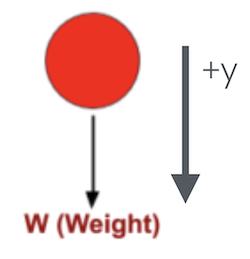
\includegraphics[keepaspectratio,alt={FBD of a falling ball}]{/Users/caballero/repos/teaching/modern-classical-mechanics/images/notes/week3/1d-ball-fbd.png}}
\caption{FBD of a falling ball}
\end{figure}

We can apply Newton's laws to obtain the specific EOM for the ball.

\[\vec{F}_{\text{net}} = m \vec{a} = m\ddot{\vec{x}}\]

This is a 1D case in the \(y\) direction,

\[F_{\text{net,y}} = W = mg = m \ddot{y}\]

Thus,

\[\ddot{y} = g\]

is the specific EOM for the ball.

\subsubsection{Example: Simple Harmonic
Oscillator}\label{example-simple-harmonic-oscillator}

We will spend a lot of time studying the
\href{https://en.wikipedia.org/wiki/Harmonic_oscillator}{simple harmonic
oscillator} (SHO) in this course. The SHO is a system that oscillates
back and forth around an equilibrium position. It is a very common
system in physics and is used a base model for many more complex
systems. Consider a mass, \(m\), attached to a spring with spring
constant, \(k\), sitting on a frictionless horizontal plane as in the
figure below.

\begin{figure}
\centering
\pandocbounded{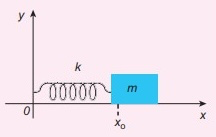
\includegraphics[keepaspectratio,alt={FBD of a simple harmonic oscillator}]{/Users/caballero/repos/teaching/modern-classical-mechanics/images/notes/week3/sho_horizontal.png}}
\caption{FBD of a simple harmonic oscillator}
\end{figure}

The EOM for the SHO can be derived form Newton's Second Law.

\[\vec{F}_{\text{net}} = m \vec{a} = m\ddot{\vec{x}}\]

This is a 1D case in the \(x\) direction,

\[F_{\text{net,x}} = F_{\text{spring}} = -kx = m \ddot{x}\]

And thus,

\[\ddot{x} = -\dfrac{k}{m}x\]

is the specific EOM for the SHO. As we will learn, this restoring force
causes the mass to oscillate back and forth around the equilibrium
position, with a well known frequency, \(\omega = \sqrt{\dfrac{k}{m}}\).

    \subsection{Turning Observations into
Models}\label{turning-observations-into-models}

One of the more challenging aspects of physics is how we work to make
models of the observations we have. This a long and challenging process
in general, but if we have a general schematic, we can make progress.
The hand drawn figure below provides such a schematic.

\begin{figure}
\centering
\pandocbounded{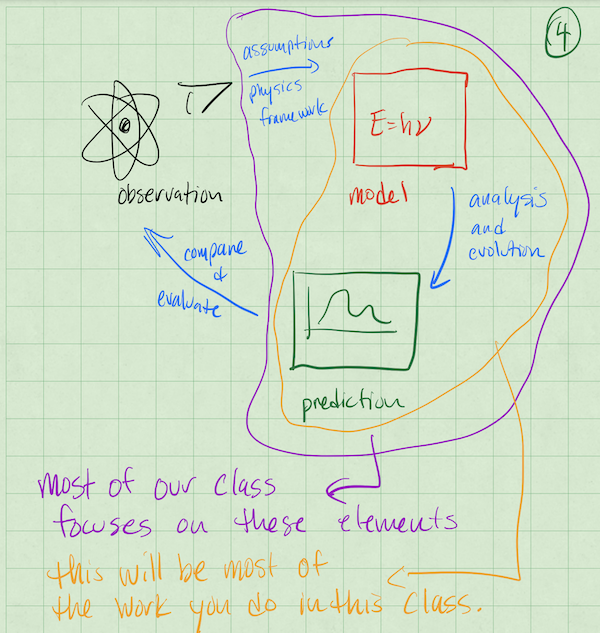
\includegraphics[keepaspectratio,alt={Framework for making models}]{/Users/caballero/repos/teaching/modern-classical-mechanics/images/notes/week3/prelim_framework.png}}
\caption{Framework for making models}
\end{figure}

In the schematic, our observations are the starting point. Using our
framework for physics (e.g., Newton's Laws) and making the appropriate
assumptions (in blue), we can develop a model (in red) of the system. By
conducting analysis and investgating the evolution of the model, we
produce predictions (in green). We can then compare tose predictions to
our observations to evaluate how well our model describes the system.

In this class, we mostly focus on the elements circled in purple where
we develop models, and use them to predict. The core part of this class
is the orange circled elements of modeling and predicting. We will spend
a lot of time developing the tools and techniques to make these
predictions.

\subsubsection{Modeling Process}\label{modeling-process}

Making models of physical systems is greatly helped by considering the
following steps:

\begin{itemize}
\tightlist
\item
  Identify the phenomenon or system of interest.
\item
  Identify the interactions the system has with its surroundings.
\item
  Choose an appropriate physics framework to investigate the system
  (Newton? Lagrange? Hamilton? Continuous or Discrete?).
\item
  Sketch the system and identify the interactions, name them, and assign
  them to the appropriate framework.
\item
  Choose your coordinate system and define your variables.
\item
  Apply the appropriate physics framework to the system.
\item
  \textbf{Obtain the equations of motion}, and make predictions.
\end{itemize}

Let's turn to an example you have seen before: the falling ball.

    \subsubsection{Example: Falling Ball in
1D}\label{example-falling-ball-in-1d}

Consider a ball of mass \(m\) falling with air resistance. Here, we have
already done some of the work above. We have identified the phenomenon,
and started to indicate the interactions.

\begin{figure}
\centering
\pandocbounded{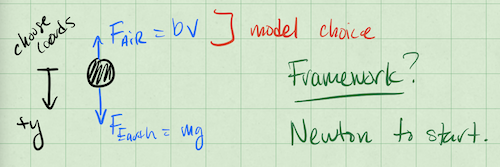
\includegraphics[keepaspectratio,alt={FBD of a falling ball with air resistance}]{/Users/caballero/repos/teaching/modern-classical-mechanics/images/notes/week3/1d-ball-fbd-air.png}}
\caption{FBD of a falling ball with air resistance}
\end{figure}

In the figure above, we have identified the forces acting on the ball.
We have the gravitational force, \(W = mg\), and the air resistance,
\(F_{\text{air}}\). We have chosen the linear mode for air-resistance,
which is a choice of model given the assumption that the ball moves very
slowly -- \emph{this is not a good assumption in this case}, but makes
the mathematical analysis simpler.

We have also chosen our coordinate system, with the positive \(y\)
direction pointing down.

We choose a Newtonian framework for our physics because we are familiar
with it. And thus, we can develop the EOM:

\[\vec{F}_{\text{net}} = m \vec{a} = m\ddot{\vec{x}}\]

In 1d,

\[F_{\text{net,y}} = W - F_{\text{air}} = mg - bv = m \ddot{y}\]

So that the EOM is,

\[\ddot{y} = g - \dfrac{b}{m}v\]

\paragraph{\texorpdfstring{Question: What happens with
\(\ddot{y} = 0\)?}{Question: What happens with \textbackslash ddot\{y\} = 0?}}\label{question-what-happens-with-ddoty-0}

Once the ball has no acceleration, the two forces are balanced. This is
the terminal velocity of the ball. We can solve for this by setting
\(\ddot{y} = 0\):

\[0 = g - \dfrac{b}{m}v_{\text{term}}\]

\[v_{\text{term}} = \dfrac{mg}{b}\]

This is the terminal velocity of the ball for linear drag. When the ball
reaches this speed (and does so asymptotically), the forces are balanced
and the ball will fall at a constant speed.

\paragraph{Question can we solve this differential
equation?}\label{question-can-we-solve-this-differential-equation}

The differential equation \(\ddot{y} = g - \dfrac{b}{m}v\) is a
second-order differential equation for \(y\). We can solve this equation
analytically by recasting it as a first-order differential equation for
\(v\), which we solve for and then integrate to find \(y(t)\).

\[\dot{v} = g - \dfrac{b}{m}v\]

We will do that later, for now, let's hack off the drag bit and return
to the simple falling ball. Our simplified EOM is:

\[\ddot{y} = g\]

Note this is written as a second order ODE for \(y\):

\[\dfrac{d^2y}{dt^2} = g\]

It is possible also to recast these kinds of second-order differential
equations as a pair of 1st order differential equations for \(y\) and
\(v\):

\[\dfrac{dv}{dt} = g \qquad \dfrac{dy}{dt} = v\]

This is a common technique in physics and engineering to solve
second-order differential equations. Let's solve this for completeness.

\[\dfrac{dv}{dt} = g \longrightarrow \textrm{a constant}\]

We can integrate:

\[\int_{v_0}^{v(t)} dv = \int_{0}^{t} g dt\]

\[v(t) - v_0 = gt\]

We obtain the velocity as a function of time for constant acceleration:

\[v(t) = v_0 + gt\]

Now we can integrate the velocity to obtain the position as a function
of time:

\[\dfrac{dy}{dt} = v \longrightarrow \textrm{a function of time}\]

\[\int_{y_0}^{y(t)} dy = \int_{0}^{t} v_0 + gt dt\]

\[y(t) - y_0 = v_0 t + \dfrac{1}{2}gt^2\]

We obtain the position as a function of time for constant acceleration,
the standard kinematic equation:

\[y(t) = y_0 + v_0 t + \dfrac{1}{2}gt^2\]

Why the `plus' sign on the last term? Because we choose positive \(y\)
to be down, and the ball is accelerating down.

\texttt{\{note\}\ This\ is\ really\ useful,\ but\ is\ contingent\ on\ finding\ or\ knowing\ the\ anti-derivative\ of\ the\ functions\ we\ are\ integrating.\ That\ is\ not\ always\ possible.\ What\ might\ we\ do\ if\ we\ weren\textquotesingle{}t\ sure\ that\ we\ could\ find\ the\ anti-derivative?}

    \subsection{Discrete Formulation of Newtonian
Mechanics}\label{discrete-formulation-of-newtonian-mechanics}

Most of our experience so far has been solving problems where we can
find continuous functions that are the anti-derivatives of the functions
we are integrating. This leads to standard formulae that we can use to
predict or plot our results.

However, there are very few systems for which we can write down EOMs
that have known solutions. In these cases, we need to turn to numerical
methods to solve the equations of motion. To do this, we need a discrete
formulation of the EOMs.

Let's focus on 1D:

\[\dfrac{d^2y}{dt^2} = \dfrac{F}{m}\]

We can write this as a pair of first-order differential equations:

\[\dfrac{dy}{dt} = v \quad \textrm{and} \quad \dfrac{dv}{dt} = \dfrac{F}{m}\]

Let's allow ourselves to consider instead a small time interval of the
evolution, \(\Delta t\). We can then write the velocity equation as:

\[\dfrac{dv}{dt} = \dfrac{\Delta v}{\Delta t}= \dfrac{v(t+\Delta t) - v(t)}{\Delta t} = \dfrac{F}{m}\]

We can turn this into a discrete equation by multiplying through by
\(\Delta t\): prediction of the velocity at the next time step:

\[v(t+\Delta t) = v(t) + \dfrac{F}{m} \Delta t\]

This is the ``velocity update'' equation, or more generally, the
\href{https://en.wikipedia.org/wiki/Euler_method}{Euler step} for
velocity. Given the information at time \(t\), \(F(t)\), \(m\), and
\(v(t)\), we can predict the velocity at the next time step.

\[v(t+\Delta t) = v(t) + \dfrac{F(t)}{m} \Delta t\]

Great! But that is just for velocity, can we do the same for position?

\textbf{Yes}

We can use the same logic to predict the position at the next time step:

\[\dfrac{dy}{dt} = v\]

If we discretize this, we realize we just have the definition of the
average velocity:

\[\dfrac{dy}{dt} = v_{\textrm{avg}}\]

We can then write the position update equation:

\[y(t+\Delta t) = y(t) + v_{\textrm{avg}} \Delta t\]

    What is left is to determine what should be the estimate for
\(v_{\textrm{avg}}\).

```\{admonition\} Choosing \(v_{\textrm{avg}}\) :class: note

The idea that we have to pick a value for \(v_{\textrm{avg}}\) is a key
point in numerical methods. It might seem silly or overly subtle and it
certainly the latter. We can select \(v(t)\), \(v(t+\Delta t)\), or some
average of the two. The choice of \(v_{\textrm{avg}}\) is the key to the
accuracy of the method.

As we will show in a later homework, the best choice is
\(v(t+\Delta t)\) as it preserves the energy of the system. ```

    \subsubsection{Euler-Cromer Step}\label{euler-cromer-step}

Taken together, we obtain the
\href{https://en.wikipedia.org/wiki/Semi-implicit_Euler_method}{Euler-Cromer}
step for the position and velocity:

\[v(t+\Delta t) = v(t) + \dfrac{F(t)}{m} \Delta t\]
\[y(t+\Delta t) = y(t) + v(t+\Delta t) \Delta t\]

This method was accidentaly discovered by a high physics student called
Abby Aspel. It was later explored by
\href{https://en.wikipedia.org/wiki/Alan_Cromer}{Alan Cromer} whote
wrote up this
\href{https://aapt.scitation.org/doi/10.1119/1.10903}{method in the
American Journal of Physics}.

In three-dimensions, this method is simply written in a vector form:

\[\vec{v}(t+\Delta t) = \vec{v}(t) + \dfrac{\vec{F}(t)}{m} \Delta t\]
\[\vec{r}(t+\Delta t) = \vec{r}(t) + \vec{v}(t+\Delta t) \Delta t\]

    ```\{admonition\} Erasing Contributions in Physics :class: note This
method should be called the Euler-Aspel-Cromer method because Euler
started it, Aspel discovered it, and Cromer formalized it.

It is not because physics and physicists tend to erase the contributions
of marginalized groups including young people, women, and folks from
non-dominant groups.

\textbf{Don't believe it?}

Read about the
\href{https://physics.mit.edu/about-physics/our-history/}{history of the
MIT physics department} and try to find the contributions of the many
technical staff, non-tenure track faculty, and students who have made
the department what it is today. ```

    \subsection{Analytical Solutions to the Air-Resistance
Problem}\label{analytical-solutions-to-the-air-resistance-problem}

We can solve the air-resistance problem analytically. We have the EOM
for velocity:

\[\dot{v} = g - \dfrac{b}{m}v - \dfrac{c}{m}v^2\]

\subsubsection{Linear Drag}\label{linear-drag}

Let's take the linear limit first, \(c=0\).

\[\dot{v} = g - \dfrac{b}{m}v\]

We can solve this equation by separating variables:

\[\dfrac{dv}{g - \dfrac{b}{m}v} = dt\]

We can integrate both sides:

\[\int \dfrac{dv}{g - \dfrac{b}{m}v} = \int dt\]

\[-\dfrac{m}{b} \ln|g - \dfrac{b}{m}v| = t + C\]

We can solve for \(v(t)\):

\[g - \dfrac{b}{m}v = e^{-\dfrac{b}{m}t - C}\]

\[v(t) = \dfrac{mg}{b} - e^{-\dfrac{b}{m}t - C}\]

We can solve for the constant \(C\) by using the initial condition
\(v(0) = v_0\):

\[v_0 = \dfrac{mg}{b} - e^{-C}\]

\[e^{-C} = \dfrac{mg}{b} - v_0\]

\[v(t) = \dfrac{mg}{b} - \left(\dfrac{mg}{b} - v_0\right)e^{-\dfrac{b}{m}t}\]

When \(v_0 = 0\), we find:

\[v(t) = \dfrac{mg}{b}\left(1 - e^{-\dfrac{b}{m}t}\right)\]

And as \(t \to \infty\), we find the terminal velocity:

\[v_{\text{term}} = \lim_{t \to \infty} v(t) = \dfrac{mg}{b}\]

    \subsubsection{Quadratic Drag}\label{quadratic-drag}

In the case of quadratic drag, we have:

\[\dot{v} = g - \dfrac{c}{m}v^2\]

We can find the terminal velocity by setting \(\dot{v} = 0\):

\[0 = g - \dfrac{c}{m}v_{\text{term}}^2\]

\[v_{\text{term}} = \sqrt{\dfrac{mg}{c}}\]

Thus, we recast the problem in terms of the terminal velocity:

\[\dot{v} = g\left(1 - \dfrac{v^2}{v_{\text{term}}^2}\right)\]

We can separate variables and integrate:

\[\int \dfrac{dv}{1 - \dfrac{v^2}{v_{\text{term}}^2}} = \int g dt\]

\paragraph{\texorpdfstring{Assume we start at rest,
\(v(0) = 0\)}{Assume we start at rest, v(0) = 0}}\label{assume-we-start-at-rest-v0-0}

We can solve for \(v(t)\), by using the proper limits:

\[\int_{0}^{v(t)} \dfrac{dv}{1 - \dfrac{v^2}{v_{\text{term}}^2}} = \int_{0}^{t} g dt\]

This is a known integral and yields:

\[\dfrac{v_{\text{term}}}{2}\ln\left|\dfrac{v_{\text{term}} + v}{v_{\text{term}} - v}\right| = gt\]

With the initial condition \(v(0) = 0\), we find:

\[\dfrac{v_{\text{term}}}{g} \tanh^{-1}\left(\dfrac{v}{v_{\text{term}}}\right) = t\]

And thus, we find the velocity as a function of time:

\[v(t) = v_{\text{term}}\tanh\left(\dfrac{gt}{v_{\text{term}}}\right)\]

    \begin{tcolorbox}[breakable, size=fbox, boxrule=1pt, pad at break*=1mm,colback=cellbackground, colframe=cellborder]
\prompt{In}{incolor}{ }{\boxspacing}
\begin{Verbatim}[commandchars=\\\{\}]

\end{Verbatim}
\end{tcolorbox}

    


    % Add a bibliography block to the postdoc
    
    
    
\end{document}
